\documentclass[12pt,a4paper]{article}
\usepackage[UTF8]{ctex}
\usepackage{amsmath,amssymb}
\usepackage{xcolor}
\usepackage{hyperref}
\usepackage{geometry}
\usepackage{graphicx}
\geometry{margin=2.5cm}

\title{Classical If / 经典条件分支}
\author{QuoNic}
\date{}

\begin{document}
\maketitle

\begin{center}
\textbf{Language / 语言特性} | 难度：初级 | 预计时间：5 分钟
\end{center}

\tableofcontents
\newpage

\section{为什么需要？}

经典条件分支是在量子程序中使用经典 if 语句。

\subsection{经典局限}
\begin{itemize}
  \item 经典条件分支无法直接用于量子态
  \item 需要先测量量子态
\end{itemize}

\subsection{量子优势}
\begin{itemize}
  \item 经典条件分支可以在量子程序中使用经典逻辑
  \item 是混合编程模型的基础
  \item 支持量子-经典混合算法
\end{itemize}

\subsection{实际应用}
\begin{itemize}
  \item 量子-经典混合算法
  \item 变分量子算法
  \item 量子优化
\end{itemize}

\section{快速上手}

\begin{verbatim}
from quonic import qgate, cshow
from quonic.gates import H

# 经典条件分支
qgate(H, 0)
result = cshow()
if result == '0':
    print('Measured 0')
else:
    print('Measured 1')
\end{verbatim}

\textbf{预期输出}：
\begin{verbatim}
Measured 0 (or Measured 1, with 50% probability each)
\end{verbatim}

\section{原理详解}

\subsection{电路图}

\begin{center}
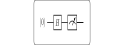
\includegraphics[width=0.6\textwidth]{../../images/cif_circuit.svg}
\end{center}

\subsection{数学推导}

经典条件分支：
\begin{equation}
\text{if } m == 0: \text{ do } A \text{ else: do } B
\end{equation}

其中 $m$ 是测量结果。

\subsection{几何解释}

经典条件分支在测量后根据经典结果执行不同操作。测量会塌缩量子态，然后根据经典变量执行经典逻辑。

\section{代码详解}

\begin{verbatim}
from quonic import qgate, cshow
from quonic.gates import H

# cshow() 返回经典测量结果
qgate(H, 0)
result = cshow()

# 经典条件分支
if result == '0':
    print('Measured 0')
else:
    print('Measured 1')
\end{verbatim}

\section{进阶用法}

\subsection{场景 1：VQE 优化循环}

\begin{verbatim}
from quonic import qgate, cshow
from quonic.gates import Ry

# VQE 优化循环
for epoch in range(100):
    qgate(Ry(theta), 0)
    result = cshow()
    energy = compute_energy(result)
    theta = update_theta(theta, energy)
\end{verbatim}

\subsection{场景 2：量子-经典混合算法}

\begin{verbatim}
from quonic import qgate, cshow
from quonic.gates import H, CX

# 量子-经典混合算法
qgate(H, 0)
qgate(CX, 0, 1)
result = cshow()

# 经典后处理
if result == '00' or result == '11':
    print('Entangled')
else:
    print('Not entangled')
\end{verbatim}

\section{适用场景}

\subsection{量子-经典混合算法}

经典条件分支用于量子-经典混合算法中的经典逻辑。例如，VQE、QAOA 等变分算法需要经典优化循环。

\subsection{量子优化}

经典条件分支用于量子优化中的参数更新。根据测量结果更新优化参数。

\section{常见问题}

\subsection{经典条件分支和量子条件分支有什么区别？}

经典条件分支基于经典变量，量子条件分支基于量子测量结果。经典条件分支不会破坏量子态。

\subsection{经典条件分支会破坏量子态吗？}

不会。经典条件分支基于经典变量，不涉及量子测量。

\section{学习路径}

\subsection{前置知识}
\begin{itemize}
  \item 量子测量
  \item 经典编程
  \item 量子比特
\end{itemize}

\subsection{继续学习}
\begin{itemize}
  \item 量子条件分支（qif）
  \item 变分量子算法
  \item 量子-经典混合算法
\end{itemize}

\section{完整示例代码}

\subsection{示例 1：基本经典条件分支}

\begin{verbatim}
from quonic import qgate, cshow
from quonic.gates import H

qgate(H, 0)
result = cshow()
if result == '0':
    print('Measured 0')
else:
    print('Measured 1')
\end{verbatim}

\section{下载}

\begin{itemize}
  \item [cif.py](https://github.com/ChrisLee0721/QuoNic/blob/main/examples/cif/cif.py)
\end{itemize}

\end{document}
